\documentclass[a4paper]{jpconf}
\usepackage{graphicx}
\usepackage{fixltx2e}

\graphicspath{{pics/}}

\newcommand{\dd}[1]{\mathrm{d}#1}

\begin{document}
\title{A Vision and GPS Based System for Autonomous Vertical Landing of UAV Quadcopter}

\author{A S Priambodo\textsuperscript{1}, F Arifin\textsuperscript{2}, A Nasuha\textsuperscript{3}, Muslikhin\textsuperscript{4}, A Winursito\textsuperscript{5}}

\address{\textsuperscript{1,2,3,4,5}Department of Electronics and Informatics Engineering of Education, Engineering Faculty, Universitas Negeri Yogyakarta, Indonesia}

\ead{ardyseto@uny.ac.id}

\begin{abstract}
    All articles {\it must} contain an abstract. This document describes the  preparation of a conference paper to be published in \jpcs\ using \LaTeXe\ and the \cls\ class file. The abstract text should be formatted using 10 point font and indented 25 mm from the left margin. Leave 10 mm space after the abstract before you begin the main text of your article. The text of your article should start on the same page as the abstract. The abstract follows the addresses and should give readers concise information about the content of the article and indicate the main results obtained and conclusions drawn. As the abstract is not part of the text it should be complete in itself; no table numbers, figure numbers, references or displayed mathematical expressions should be included. It should be suitable for direct inclusion in abstracting services and should not normally exceed 200 words. The abstract should generally be restricted to a single paragraph. Since contemporary information-retrieval systems rely heavily on the content of titles and abstracts to identify relevant articles in literature searches, great care should be taken in constructing both.
\end{abstract}

\section{Introduction}
Unmanned Aerial Vehicle (UAVs) or Drones is a topic of great interest to researchers now. A drone can do much work. In agriculture, drones are used as sprinklers of liquid fertilizer and observation of crops from the air\cite{ref1}. Drones are used as spies from the air in the military field\cite{ref2}. In the safety field, drones are used for surveillance in disaster areas\cite{ref3}. The quadcopter is one type of UAV that is widely developed because it has the advantage of being able to take off and land vertically. The quadcopter consists of four rotors that rotate the propellers to get lifts. Because the quadcopter can take off and land vertically, the required take-off area is minimal. In addition to these advantages, the quadcopter also can hover in the air.

There are various types of UAVs, namely fixed wing, rotary wing and hybrid fixed and rotary wing. In comparison, the rotary wing consists of 2 types: single rotor and multirotor. The hybrid and rotary wing UAV can take off and land vertically, so they do not require a large area. The selection of the type of UAV depends on the task and area to be completed. Multirotor has many advantages such as more agile manoeuvrability, ability to hover in the air, with a certain size, it can fly indoors, take off and land vertically and has a relatively simple frame design compared to other types. Multirotor also has disadvantages, namely limited flight time, which causes relatively small cruising area and limited carrying capacity. The multirotor that is widely developed is the quadcopter or quadrotor type. The quadcopter is a multirotor with 4 motors driving the propellers to generate lift. The quadcopter can be configured to be type X or H.

In general, flying vehicles' flight actions are based on GPS sensors. A global positioning system (GPS) is an electronic device that can be used for navigation. GPS provides latitude, longitude and altitude values as a reference from the UAV so that the UAV can fly to a certain point based on that reference. GPS on UAVs, especially quadcopters, is also used to get the take-off location and later used as a landing point. However, the GPS does not provide accurate values in some conditions and environments, so the landing becomes imprecise. In limited applications where the take-off and landing places are very narrow, this is a challenge, so we cannot just rely on GPS to find out the location of the landing point.

Manually landing a quadcopter usually has difficulties. For example, pilots find it difficult to gradually reduce the quadcopter's altitude and land smoothly and accurately at precise locations. Automatic landing using GPS is a method to facilitate the quadcopter land smoothly and accurately. However, in particular area and time conditions, the GPS accurateness becomes less good and causes the quadcopter not to land in the accurately determined area\cite{ref4}. In this paper, we propose a new automatic landing method based on GPS and computer vision so that the quadcopter can land precisely in the specified area. The take-off and landing area used in this study is an aruco marker. Improved landing accuracy, safety and reliability are the advantages of our proposed method.

\section{Methodology}
\subsection{Quadcopter Model}
A quadcopter is a type of flying vehicle which has four motors used to rotate the propeller. The propeller's rotation here will generate lift to raise the quadcopter. Adjusting the speed on each quadcopter motor can perform roll, pitch, yaw or vertical movements. Quadcopters with X configuration consist of front right, rear right, rear left, and front left motors, usually numbered 1,2,3 and 4. Quadcopters with an X configuration of 1,3 and 2,4 propeller pairs rotate in opposite directions, eliminating momentum and not requiring a tail rotor for counterbalance. Besides, this research uses an X configuration quadcopter because it has better stability than the + configuration.

The roll movement is influenced by the speed of the right part (1,2) and left part(3,4) motors. Pitch movement is affected by the speed of the front part (1,4) and rear part (2,3) motors. Yaw movement is influenced by combination of motors 1,3 and 2,4. The speed of the four motors on the quadcopter influences the vertical movement. The illustration of the quadcopter movement can be seen in Figure 1.

\begin{figure}[h]
    \centering
    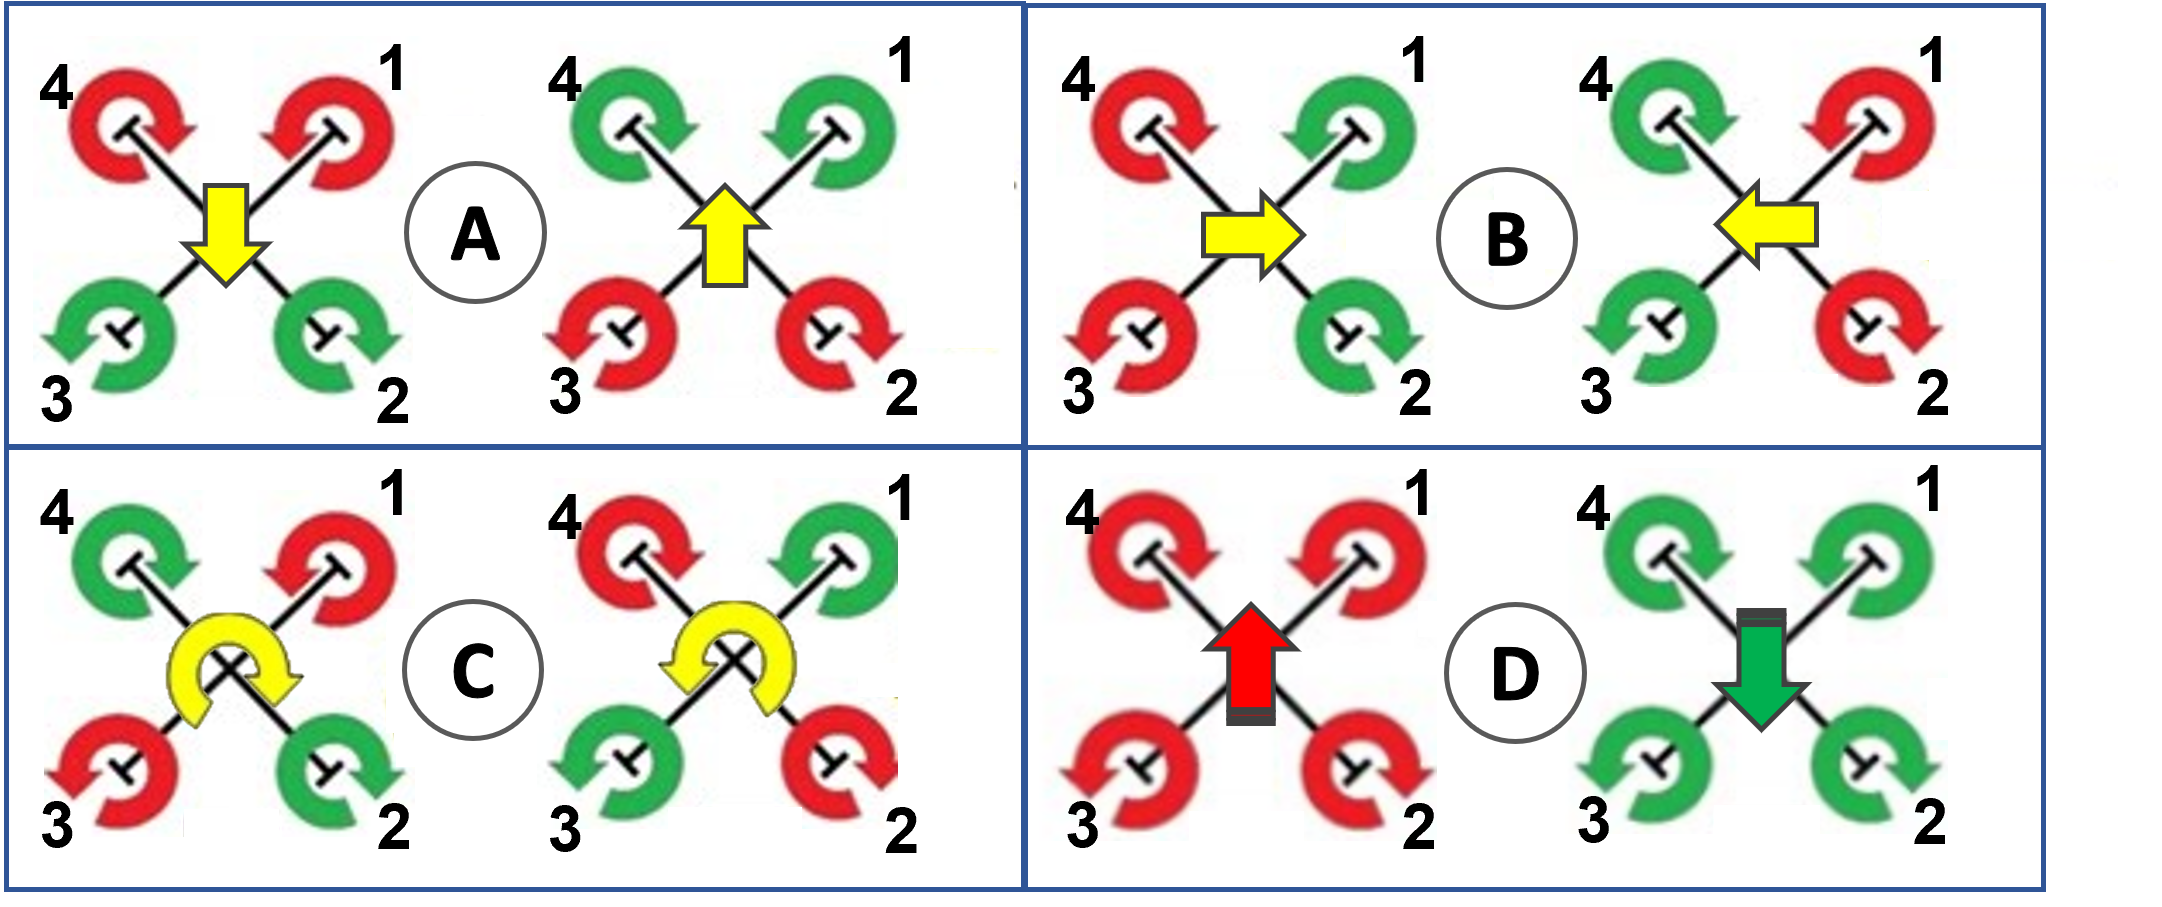
\includegraphics[width=32pc]{quadcopter-basic-movement.png}
    \caption{\label{label}Quadcopter Basic Movement: (A)Pitch (B)Roll (C)Yaw (D)Vertical Movement (the red color means faster than green)}
\end{figure}

Based on rotational and translational movements, a quadcopter mathematical model can be derived for 6-DOF using the Newton-Euler technique. Using this approach, the 6-DOF were deduced as follows:

\begin{equation}
    \ddot{\phi}=\dot{\theta}\dot{\psi}\left ( \frac{I_{y}-I_{z}}{I_{x}} \right )-\frac{J_{r}}{I_{x}}\dot{\theta}\Omega+\frac{l}{I_{x}}U_{2}
\end{equation}

\begin{equation}
    \ddot{\theta}=\dot{\phi}\dot{\psi}\left ( \frac{I_{z}-I_{x}}{I_{y}} \right )-\frac{J_{r}}{I_{y}}\dot{\phi}\Omega+\frac{l}{I_{y}}U_{3}
\end{equation}

\begin{equation}
    \ddot{\psi}=\dot{\phi}\dot{\theta}\left ( \frac{I_{x}-I_{y}}{I_{z}} \right )+\frac{l}{I_{z}}U_{4}
\end{equation}

\begin{equation}
    \ddot{x}=(cos\phi sin\theta cos\psi + sin\phi sin\psi)\frac{U_{1}}{m}
\end{equation}

\begin{equation}
    \ddot{y}=(cos\phi sin\theta cos\psi - sin\phi sin\psi)\frac{U_{1}}{m}
\end{equation}

\begin{equation}
    \ddot{z}=-g+(cos\phi cos\theta)\frac{U_{1}}{m}
\end{equation}

\subsection{Vision-Based Landing}
This study used the well-known ArUco marker as the take-off and landing area. The ArUco marker is a synthetic square marker composed of a wide black border and an inner binary matrix that defines its identifier. Black border for fast image detection and binary codification enables and application of detection and error techniques. The marker's size determines the internal matrix's size; for example, the 4x4 marker size consists of 16 bits.

\begin{figure}[h]
    \centering
    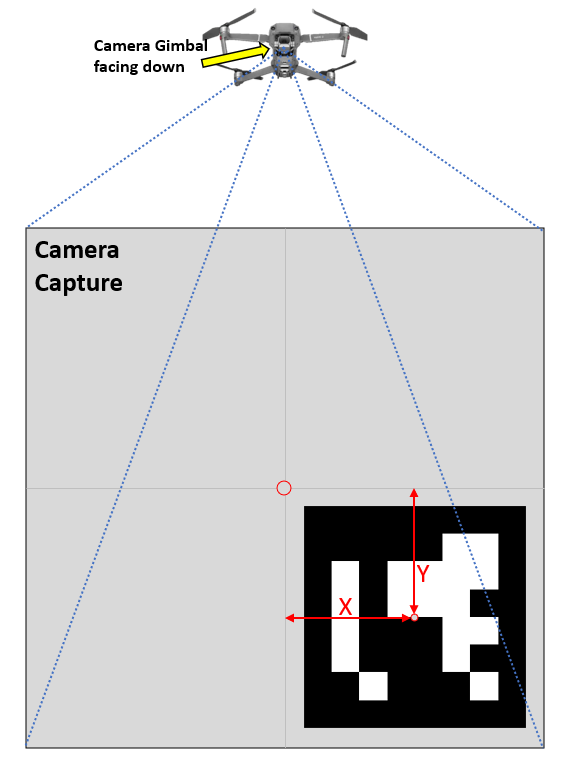
\includegraphics[width=16pc]{camera-capture-aruco.png}
    \caption{\label{label}Calculation X and Y position error based on detection of ArUco Marker}
\end{figure}

\subsection{Proposed Landing Control}
GPS is a Global Positioning System, a tool or system that can use to inform users that they are (globally) on the surface of the earth based on satellites. GPS is installed on the flight controller so the flight controller can find out where the quadcopter is. The flight controller can store the take-off position so that, theoretically, the quadcopter can land in the take-off area. In addition, GPS can also function as flying navigation at specific coordinate points.

\begin{figure}[h]
    \centering
    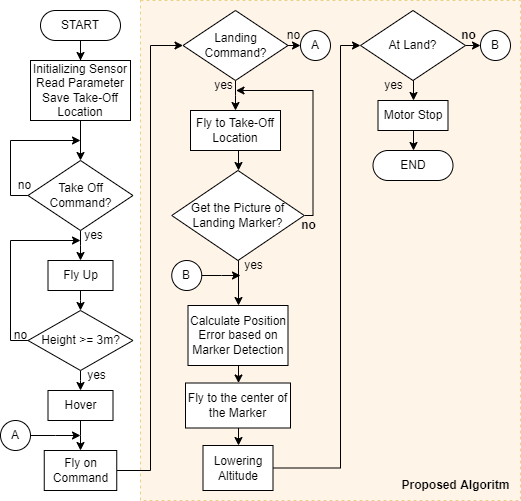
\includegraphics[width=24pc]{flowchart-proposed-algorithm.png}
    \caption{\label{label}Proposed Algorithm Flowchart of Vision and GPS Based System for Vertical Landing Quadcopter}
\end{figure}

\begin{figure}[h]
    \centering
    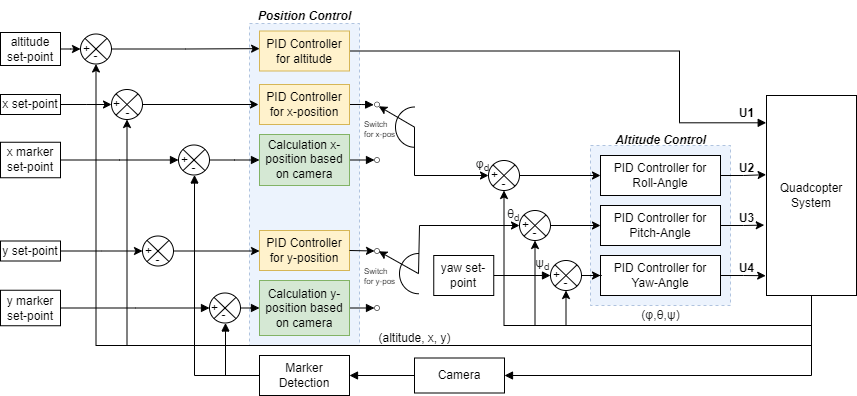
\includegraphics[width=36pc]{block-diagram-controller.png}
    \caption{\label{label}Block Diagram of Proposed Controller}
\end{figure}

\subsection{Simulation Environment}
Webots is an application or software developed by the Swiss Federal Institute of Technology that serves to create models, programs, and simulations of a robot. Using webots, we can design or design and develop programs that will run robots in an artificial environment. This application was first developed in 1996 by Dr Oliver Michael. Then in 1998, it was developed again by Cyberbotics Ltd. as proprietary licensed software. Thanks to Cyberbotics Ltd in 2018, made webots an open source application so that it is easy to use and its development becomes more available. Webots can be installed on Windows, Mac OS and Linux (Ubuntu) operating systems.

Webots provides many components in the form of robots, sensors, actuators and other objects such as humans, animals, boxes and many other things that we can use in an artificial environment. In addition, we can also create our objects through 3D CAD applications.The programming languages supported by webots also vary, namely Matlab, C/C++, Python, Java and ROS.

This study uses a DJI Mavic 2 Pro drone, in which the proposed controller will simulate a yard environment consisting of several objects such as houses, cars, roads, and many trees. The landing pad used to search at the top is displayed with the aruco marker, which the quadcopter will later recognize as the runway for landing. DJI Mavic 2 Pro consists of several sensors such as an accelerometer, gyroscope, barometer, compass and GPS that we can access through the program. The webots simulation program is run on a computer with the specifications listed in table 1.

\begin{figure}[h]
    \centering
    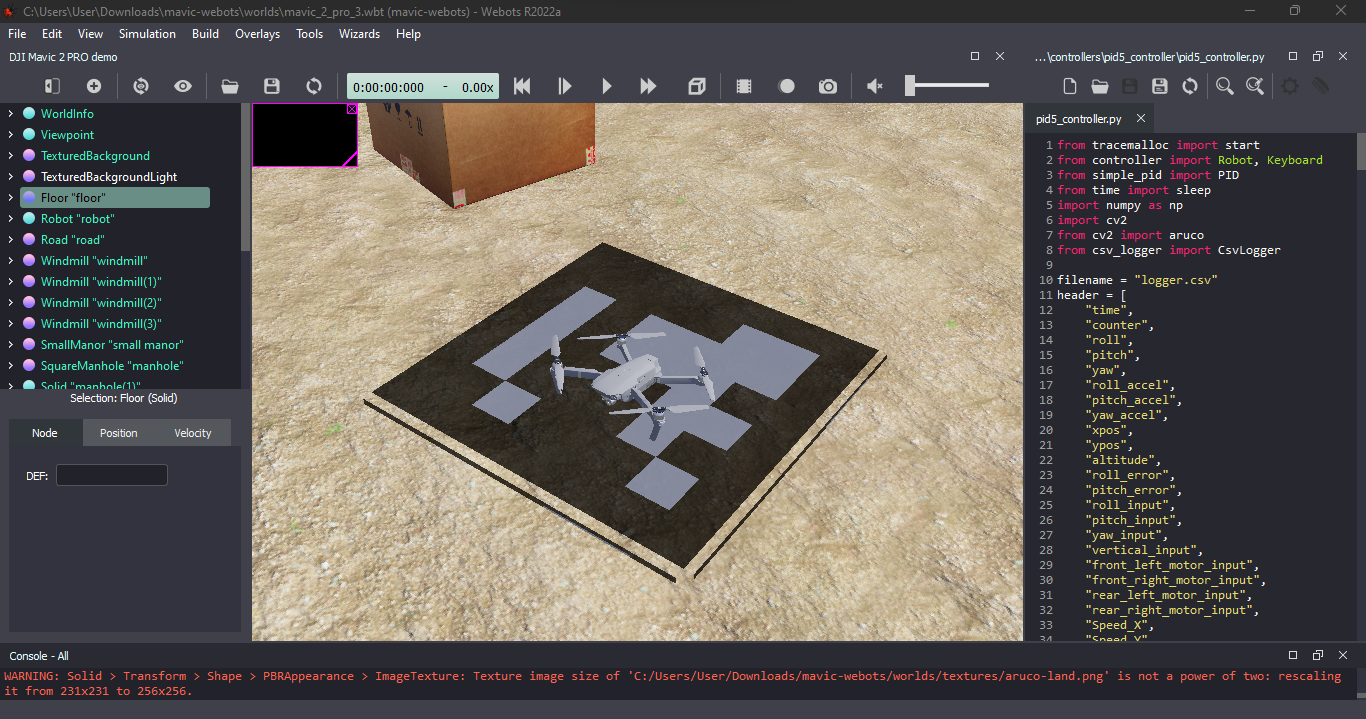
\includegraphics[width=36pc]{webots-dji-mavic-2pro.png}
    \caption{\label{label}DJI Mavic 2 Pro in Webots Environment}
\end{figure}

\begin{center}
    \begin{table}[h]
        \caption{\label{opt}Computer Spesification}
        \centering
        \begin{tabular}{@{}*{7}{l}}
            \br
            Component        & Description     \\
            \mr
            CPU              & Intel i5 12400F \\
            RAM              & 2x8GBs          \\
            GPU              & RTX 3060 12GB   \\
            Storage          & SSD NVMe Gen4x  \\
            Operating System & Ubuntu 20.04    \\
            \br
        \end{tabular}
    \end{table}
\end{center}

\section{Result and Discussion}
Authors wishing to acknowledge assistance or encouragement from
colleagues, special work by technical staff or financial support from
organizations should do so in an unnumbered Acknowledgments section
immediately following the last numbered section of the paper. The
command \verb"\ack" sets the acknowledgments heading as an unnumbered
section.

\subsection{Marker Detection}
Authors wishing to acknowledge assistance or encouragement from
colleagues, special work by technical staff or financial support from
organizations should do so in an unnumbered Acknowledgments section
immediately following the last numbered section of the paper. The
command \verb"\ack" sets the acknowledgments heading as an unnumbered
section.

\begin{figure}[h]
    \centering
    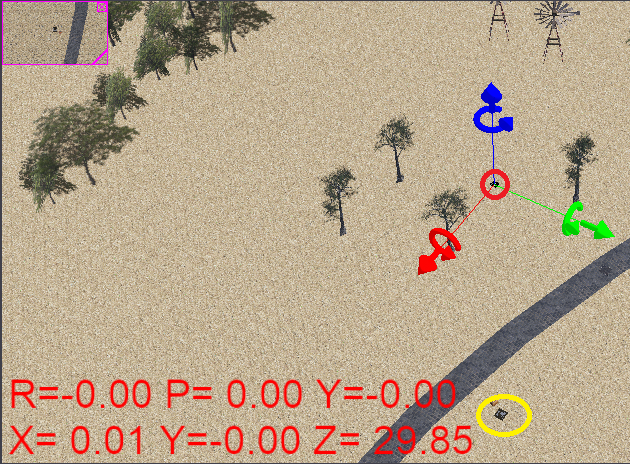
\includegraphics[width=36pc]{marker-detection-testing-edit.png}
    \caption{\label{label}Marker detecion testing in Webots. There is information about the translational and rotational position of the quadcopter which is displayed in red font. The quadcopter is marked with a red circle and the aruco marker is marked with an yellow circle.}
\end{figure}

\begin{figure}[h]
    \centering
    \begin{minipage}{15pc}
        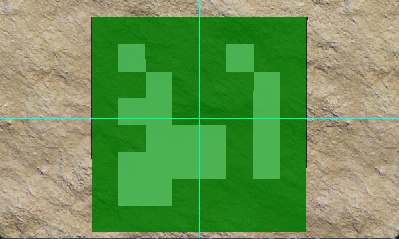
\includegraphics[width=16pc]{aruco-at-2m.png}
        \caption{\label{label}Detection of ArUco marker at a distance of 2.17 meters}
    \end{minipage}\hspace{2pc}%
    \begin{minipage}{15pc}
        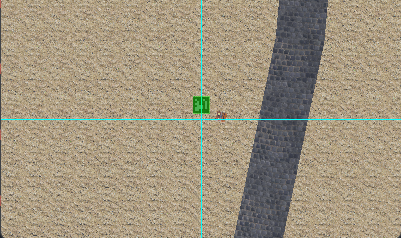
\includegraphics[width=16pc]{aruco-at-29m.png}
        \caption{\label{label}Detection of ArUco marker at a distance of 29.05 meters}
    \end{minipage}
\end{figure}

\subsection{Precision Landing}
Authors wishing to acknowledge assistance or encouragement from
colleagues, special work by technical staff or financial support from
organizations should do so in an unnumbered Acknowledgments section
immediately following the last numbered section of the paper. The
command \verb"\ack" sets the acknowledgments heading as an unnumbered
section.

\section{Conclusion}
Authors wishing to acknowledge assistance or encouragement from
colleagues, special work by technical staff or financial support from
organizations should do so in an unnumbered Acknowledgments section
immediately following the last numbered section of the paper. The
command \verb"\ack" sets the acknowledgments heading as an unnumbered
section.

\section*{Acknowledgments}
This work was supported by the Group Research Research Grant for the BEAIS Research Group in 2021 which was funded by DIPA Yogyakarta State University, Indonesia, Contract Number XXX

\section*{References}
\begin{thebibliography}{9}
    \bibitem{ref1} IOP Publishing is to grateful Mark A Caprio, Center for Theoretical Physics, Yale University, for permission to include the {\tt iopart-num} \BibTeX package (version 2.0, December 21, 2006) with  this documentation. Updates and new releases of {\tt iopart-num} can be found on \verb"www.ctan.org" (CTAN).

    \bibitem{ref2} IOP Publishing is to grateful Mark A Caprio, Center for Theoretical Physics, Yale University, for permission to include the {\tt iopart-num} \BibTeX package (version 2.0, December 21, 2006) with  this documentation. Updates and new releases of {\tt iopart-num} can be found on \verb"www.ctan.org" (CTAN).

    \bibitem{ref3} IOP Publishing is to grateful Mark A Caprio, Center for Theoretical Physics, Yale University, for permission to include the {\tt iopart-num} \BibTeX package (version 2.0, December 21, 2006) with  this documentation. Updates and new releases of {\tt iopart-num} can be found on \verb"www.ctan.org" (CTAN).

    \bibitem{ref4} IOP Publishing is to grateful Mark A Caprio, Center for Theoretical Physics, Yale University, for permission to include the {\tt iopart-num} \BibTeX package (version 2.0, December 21, 2006) with  this documentation. Updates and new releases of {\tt iopart-num} can be found on \verb"www.ctan.org" (CTAN).

    \bibitem{ref5} IOP Publishing is to grateful Mark A Caprio, Center for Theoretical Physics, Yale University, for permission to include the {\tt iopart-num} \BibTeX package (version 2.0, December 21, 2006) with  this documentation. Updates and new releases of {\tt iopart-num} can be found on \verb"www.ctan.org" (CTAN).

    \bibitem{ref6} IOP Publishing is to grateful Mark A Caprio, Center for Theoretical Physics, Yale University, for permission to include the {\tt iopart-num} \BibTeX package (version 2.0, December 21, 2006) with  this documentation. Updates and new releases of {\tt iopart-num} can be found on \verb"www.ctan.org" (CTAN).

    \bibitem{ref7} IOP Publishing is to grateful Mark A Caprio, Center for Theoretical Physics, Yale University, for permission to include the {\tt iopart-num} \BibTeX package (version 2.0, December 21, 2006) with  this documentation. Updates and new releases of {\tt iopart-num} can be found on \verb"www.ctan.org" (CTAN).

    \bibitem{ref8} IOP Publishing is to grateful Mark A Caprio, Center for Theoretical Physics, Yale University, for permission to include the {\tt iopart-num} \BibTeX package (version 2.0, December 21, 2006) with  this documentation. Updates and new releases of {\tt iopart-num} can be found on \verb"www.ctan.org" (CTAN).

    \bibitem{ref9} IOP Publishing is to grateful Mark A Caprio, Center for Theoretical Physics, Yale University, for permission to include the {\tt iopart-num} \BibTeX package (version 2.0, December 21, 2006) with  this documentation. Updates and new releases of {\tt iopart-num} can be found on \verb"www.ctan.org" (CTAN).

    \bibitem{ref10} IOP Publishing is to grateful Mark A Caprio, Center for Theoretical Physics, Yale University, for permission to include the {\tt iopart-num} \BibTeX package (version 2.0, December 21, 2006) with  this documentation. Updates and new releases of {\tt iopart-num} can be found on \verb"www.ctan.org" (CTAN).

    \bibitem{ref11} IOP Publishing is to grateful Mark A Caprio, Center for Theoretical Physics, Yale University, for permission to include the {\tt iopart-num} \BibTeX package (version 2.0, December 21, 2006) with  this documentation. Updates and new releases of {\tt iopart-num} can be found on \verb"www.ctan.org" (CTAN).

    \bibitem{ref12} IOP Publishing is to grateful Mark A Caprio, Center for Theoretical Physics, Yale University, for permission to include the {\tt iopart-num} \BibTeX package (version 2.0, December 21, 2006) with  this documentation. Updates and new releases of {\tt iopart-num} can be found on \verb"www.ctan.org" (CTAN).

    \bibitem{ref13} IOP Publishing is to grateful Mark A Caprio, Center for Theoretical Physics, Yale University, for permission to include the {\tt iopart-num} \BibTeX package (version 2.0, December 21, 2006) with  this documentation. Updates and new releases of {\tt iopart-num} can be found on \verb"www.ctan.org" (CTAN).

    \bibitem{ref14} IOP Publishing is to grateful Mark A Caprio, Center for Theoretical Physics, Yale University, for permission to include the {\tt iopart-num} \BibTeX package (version 2.0, December 21, 2006) with  this documentation. Updates and new releases of {\tt iopart-num} can be found on \verb"www.ctan.org" (CTAN).

    \bibitem{ref15} IOP Publishing is to grateful Mark A Caprio, Center for Theoretical Physics, Yale University, for permission to include the {\tt iopart-num} \BibTeX package (version 2.0, December 21, 2006) with  this documentation. Updates and new releases of {\tt iopart-num} can be found on \verb"www.ctan.org" (CTAN).

    \bibitem{ref16} IOP Publishing is to grateful Mark A Caprio, Center for Theoretical Physics, Yale University, for permission to include the {\tt iopart-num} \BibTeX package (version 2.0, December 21, 2006) with  this documentation. Updates and new releases of {\tt iopart-num} can be found on \verb"www.ctan.org" (CTAN).
\end{thebibliography}

\end{document}